\documentclass[border=10pt]{standalone}
\usepackage{pgfplots}
\pgfplotsset{compat=1.12}
\begin{document}
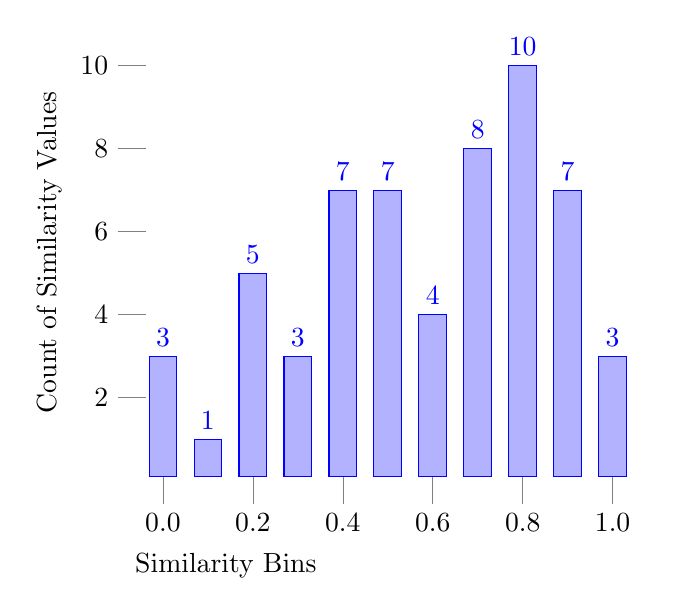
\begin{tikzpicture}
  \begin{axis}[title  = ,xlabel={Similarity Bins}, 
    ylabel={Count of Similarity Values},
    ybar,
    y axis line style = { opacity = 0},
    x axis line style = { opacity = 0},
    tickwidth = 10pt,
    nodes near coords,
    clip=false,
    ytick pos=left,
    xtick pos=left,
    symbolic x coords = {0.0,0.1,0.2,0.3,0.4,0.5,0.6,0.7,0.8,0.9,1.0},
    x label style={at={(axis description cs:0.2,-0.15)},anchor=north},
  ]
  \addplot coordinates {
  (0.0,3)
  (0.1,1) 
  (0.2,5)
  (0.3,3)
  (0.4,7)
  (0.5,7)
  (0.6,4)
  (0.7,8)
  (0.8,10)
  (0.9,7)
  (1.0,3)
  };
  \end{axis}
\end{tikzpicture}
\end{document}